%%____________________________________________________________________________||

\section{Estimation for QCD multijet events \label{sec:qcd}}

One of the major challenges for searches of new physics in the jets +
\met final state is the control of background events from QCD multijet
production. The difficulties in the determination of precise estimates
for this background stem from the large cross sections expected in the
high-energy, high-luminosity hadron collider environment at the LHC,
which are further compounded by the lack of precise theoretical
predictions for the cross sections and kinematic properties of
multijet events. Hence, without special consideration and treatment,
significant uncertainties on large background expectations can
overwhelm any potential sensitivity to new physics signatures.

With regards to QCD multijet production, the approach of this analysis
is to favour the suppression of the multijet background to a
negligible level over the goal of high efficiency for any given signal
model. A conservative uncertainty on a negligible contribution is our
preferred approach for the first analysis, over a procedure that
attempts to accurately estimate a non-negligible contribution from
multijet events. When more data are available, we might also attempt to
further lower thresholds and to establish a data-driven approach to
measure any residual multijet background in the signal region. For the
analysis, however, the level of contamination should be sufficiently
small (\ie sub-percent level) such that the associated uncertainty, even
if large, will be sub-dominant with respect to the uncertainties on the
remaining SM backgrounds with genuine \met such as \wj, \znunu, and
\ttbar, henceforth labelled as non-multijet processes.




Any contamination from QCD multijet events is controlled primarily
through the \alphat and \bdphi variables. The \alphat variable is able
to distiguish with high efficiency the sources of ``fake'' \met, such
as jet energy mismeasurement, from those with ``genuine'' \met, such
as neutrinos. The \bdphi variable is particularly efficient at
identifying jets that suffer both under- and over-measurements in
(otherwise balanced) multijet events. The variable is also
particularly suited to identifying multijet events exhibiting
significant \met due to the production of neutrinos (collinear with a
jet axis) in semileptonic heavy-flavour decays. Both variables are
capable of reducing the yields from multijet events by several orders
of magnitude.

%A couple of simple considerations can give an indication as to what
%thresholds provide adequate protection against jet threshold effects
%or QCD multijet events suffering from ``extreme'' instrumental
%effects. In the case of \bdphi, instrumental effects leading to jet
%\Pt mismeasurement will result in an \mht vector collinear in $\phi$
%with respect to the affected jet axis. In the case of heavy flavour
%decays, the neutrinos will be approximately collinear with respect to
%the jet axis. The threshold requirement on \bdphi is expected to be
%approximately similar to the anti-\kt cone size parameter value of
%0.4. In the case of \alphat, consider a balanced ``mercedes''
%three-jet event in which the jets are separated from their neighbour
%by $\Delta \phi = 120^\textrm{o}$ and each jet has a transverse energy
%of $\Et \approx x\GeV$. Assume that two jets have transverse energies
%just above a jet transverse energy threshold of $X\gev$ and the third
%falls just below. \ie, two jets satisfy $x + \delta x > X\gev$ and the
%third jet satisfies $x - \delta x > X\gev$, such that only two of the
%three jets are considered by the analysis and what was a ``balanced''
%three-jet event is considered as a dijet event with ``fake'' missing
%transerve energy from the jet below threshold. Using
%Eq. (\ref{eq:alphat3}) and in the limit $\delta x \rightarrow 0$ and
%$x \rightarrow X$, then $\scalht = 2x$, $\mht = x$, and $\dht =
%0$. Hence, Eq. (\ref{eq:alphat3}) simplifies to $\alphat =
%\frac{1}{2}\cdot\frac{1 - (0/2x)}{\sqrt{1 - (x/2x)^2}} =
%\frac{1}{2}\cdot\frac{1}{\sqrt(0.75)} = 0.577$.  In the case of a
%similarly balanced ``mercedes'' event at a higher scale, \ie when $x =
%2X$, if one jet suffers a severe undermeasurement of greater than
%50\%, then the jet will fall below the threshold $X$ and the ``full''
%\Pt (equal to $2x$) of the jet will be lost. Still, the \alphat value
%will be 0.577.  (For completeness: the case when all three jets are
%just above threshold, \ie, a perfectly balanced multijet event, then
%$\scalht = 3x$, $\mht = 0$, and $\dht = x$, hence $\alphat = 0.5$.)
%The topology described above is considered to be an extreme case of a
%multijet event generating ``fake'' \met due to a threshold effect
%(potentially compounded by a severe undermeasurement). It is important
%to note that the aforementioned requirement $\mhtmet < 1.25$ would
%likely reject this (extreme) event on the basis of a large discrepancy
%in \mht and \met. More generally, the \mhtmet variable is used to the
%filter the rare occurance in which multiple jets below threshold are
%relatively collinear in $\phi$, thus significantly biasing the \mht
%value (high) with respect to \met. 
%@@ WHAT ABOUT LOWER ALPHAT THRESHOLDS AT HIGHER HT? 
%@@ IS JET THRESHOLD EFFECT LESS IMPORTANT? 

The \alphat thresholds required to control multijet contamination to
the required level were determined by a method used in the Run~1
analysis. The method takes advantage of a multijet-enriched sidebands
in the variables \alphat and \mhtmet, the latter of which is used to
filter QCD multijet events that contain soft jets below threshold
contributing significantly to \mht. The method relies on the
exponential modelling of the number of events passing and failing a
requirement on the variable \mhtmet (\ie the pass/fail ratio \rmhtmet)
as a function of \alphat for a given signal region bin (defined in
terms of \njet, \nb, and \scalht). In essence, an ABCD approach is
used that takes into account the correlation between the variables
\rmhtmet and \alphat.

The method can be summarised as follows. The events in the sideband
are collected with the \texttt{HLT\_HTxxx} prescaled triggers
described in Sec.~\ref{sec:triggers}. Events are binned according to \alphat
and \mhtmet. Any contribution from non-multijet backgrounds in each
bin is estimated from the muon data control samples and transfer
factors determined from simulation (using the method described in
Sec.~\ref{sec:backgroundmet}) and subtracted from the data counts. Any remaining counts
are assumed to arise from multijet production. The number of counts
integrated below and above the threshold $\mhtmet = 1.25$, \ie the
pass/fail ratio \rmhtmet, is determined as a function of bins in
\alphat. The observed ratio and its dependence on \alphat is then
parameterised by an exponentially falling function in a low \alphat
sideband region and extrapolated to higher values of \alphat. An
estimate for the number of multijet events above a threshold value of
\alphat is determined by taking the product of the fit expectation and
the (non-multijet-subtracted) counts in the \mhtmet sideband. The
prediction is determined as a function of an \alphat threshold, which
is chosen when the prediction reaches the sub-percent level with
respect to the contribution from all non-multijet processes. All
relevant statistical uncertainties are propagated through to the
multijet prediction. Alternative functional forms are considered,
which are used to derive a systematic uncertainty on the multijet
prediction. 

\begin{figure}[!h]
  \centering
  \subfigure[Low \njet multiplicities.]{
    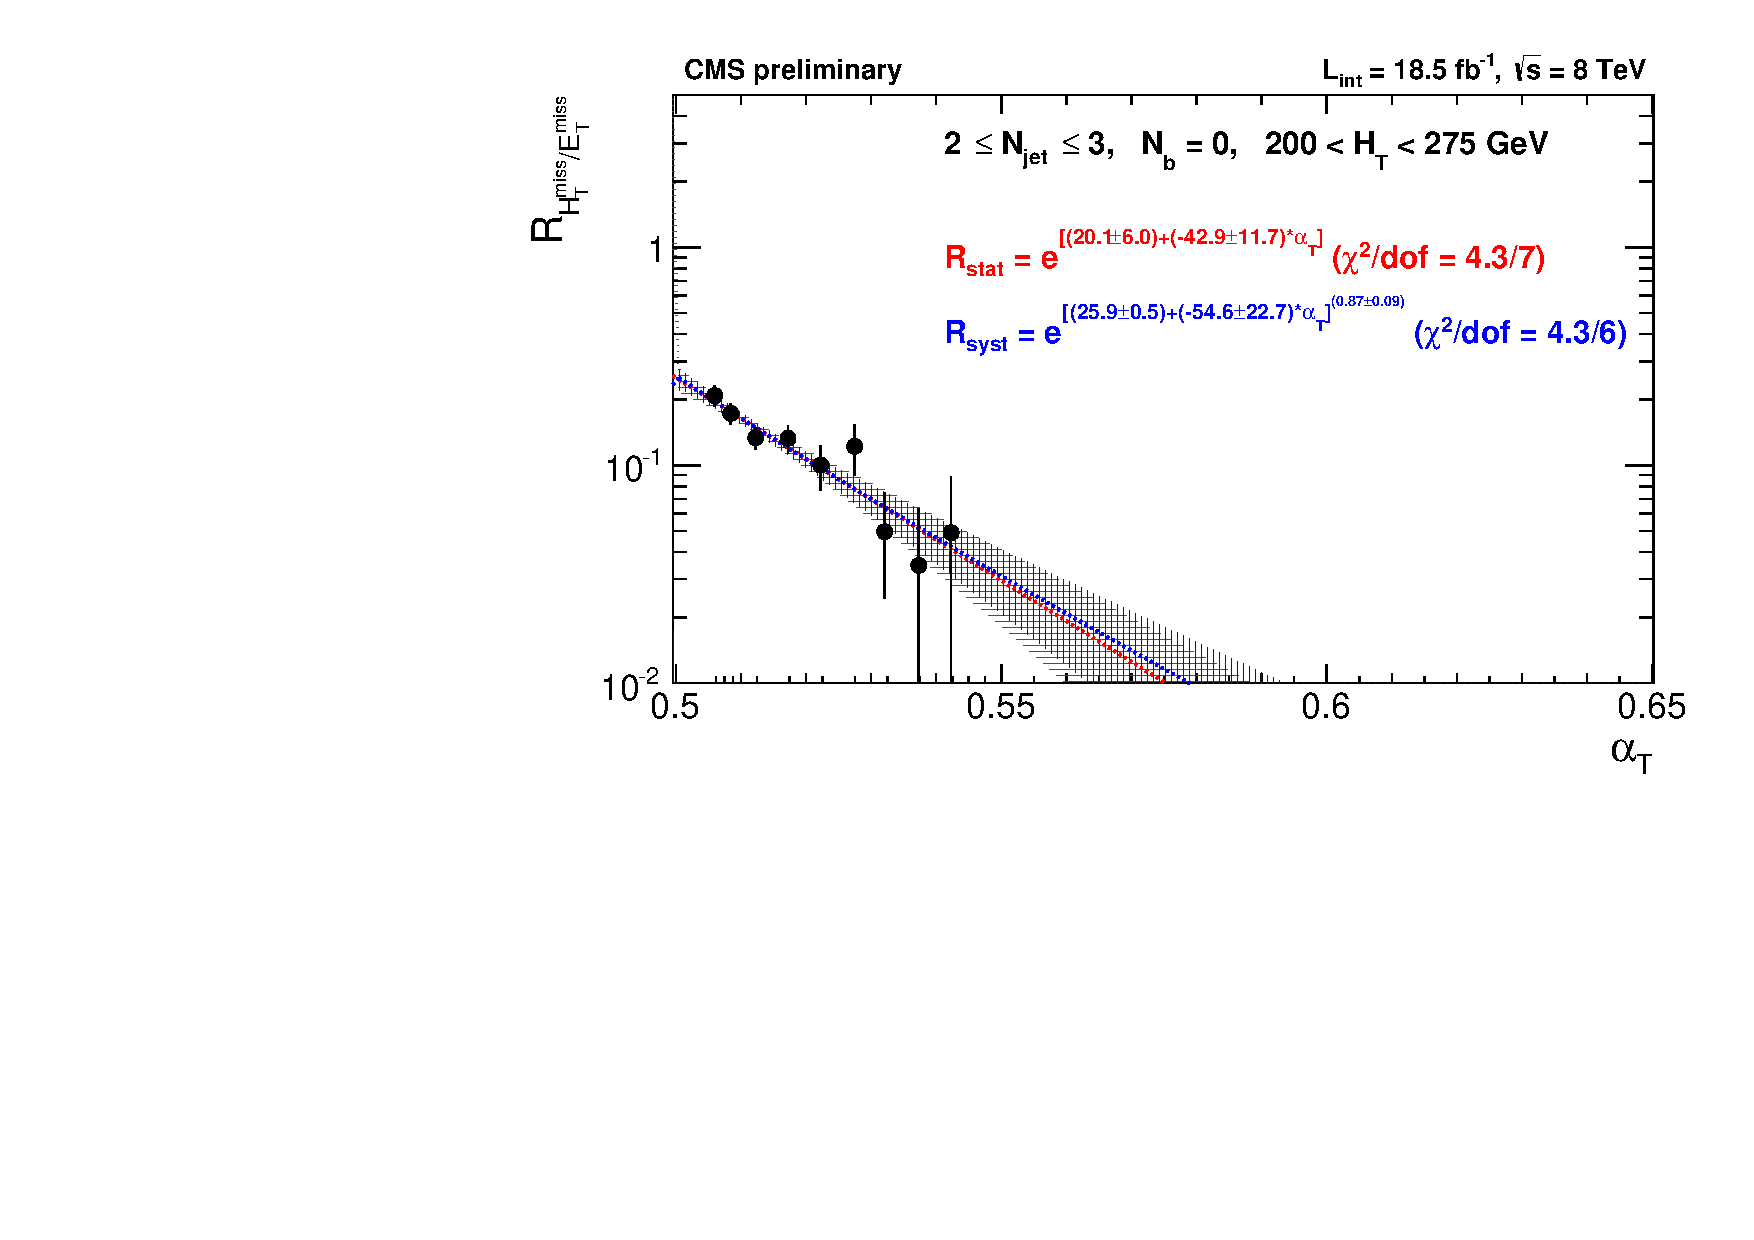
\includegraphics[width=0.5\textwidth]{figures/qcd/ratio_le3j_eq0b_200}
  } 
  \subfigure[High \njet multiplicities]{
    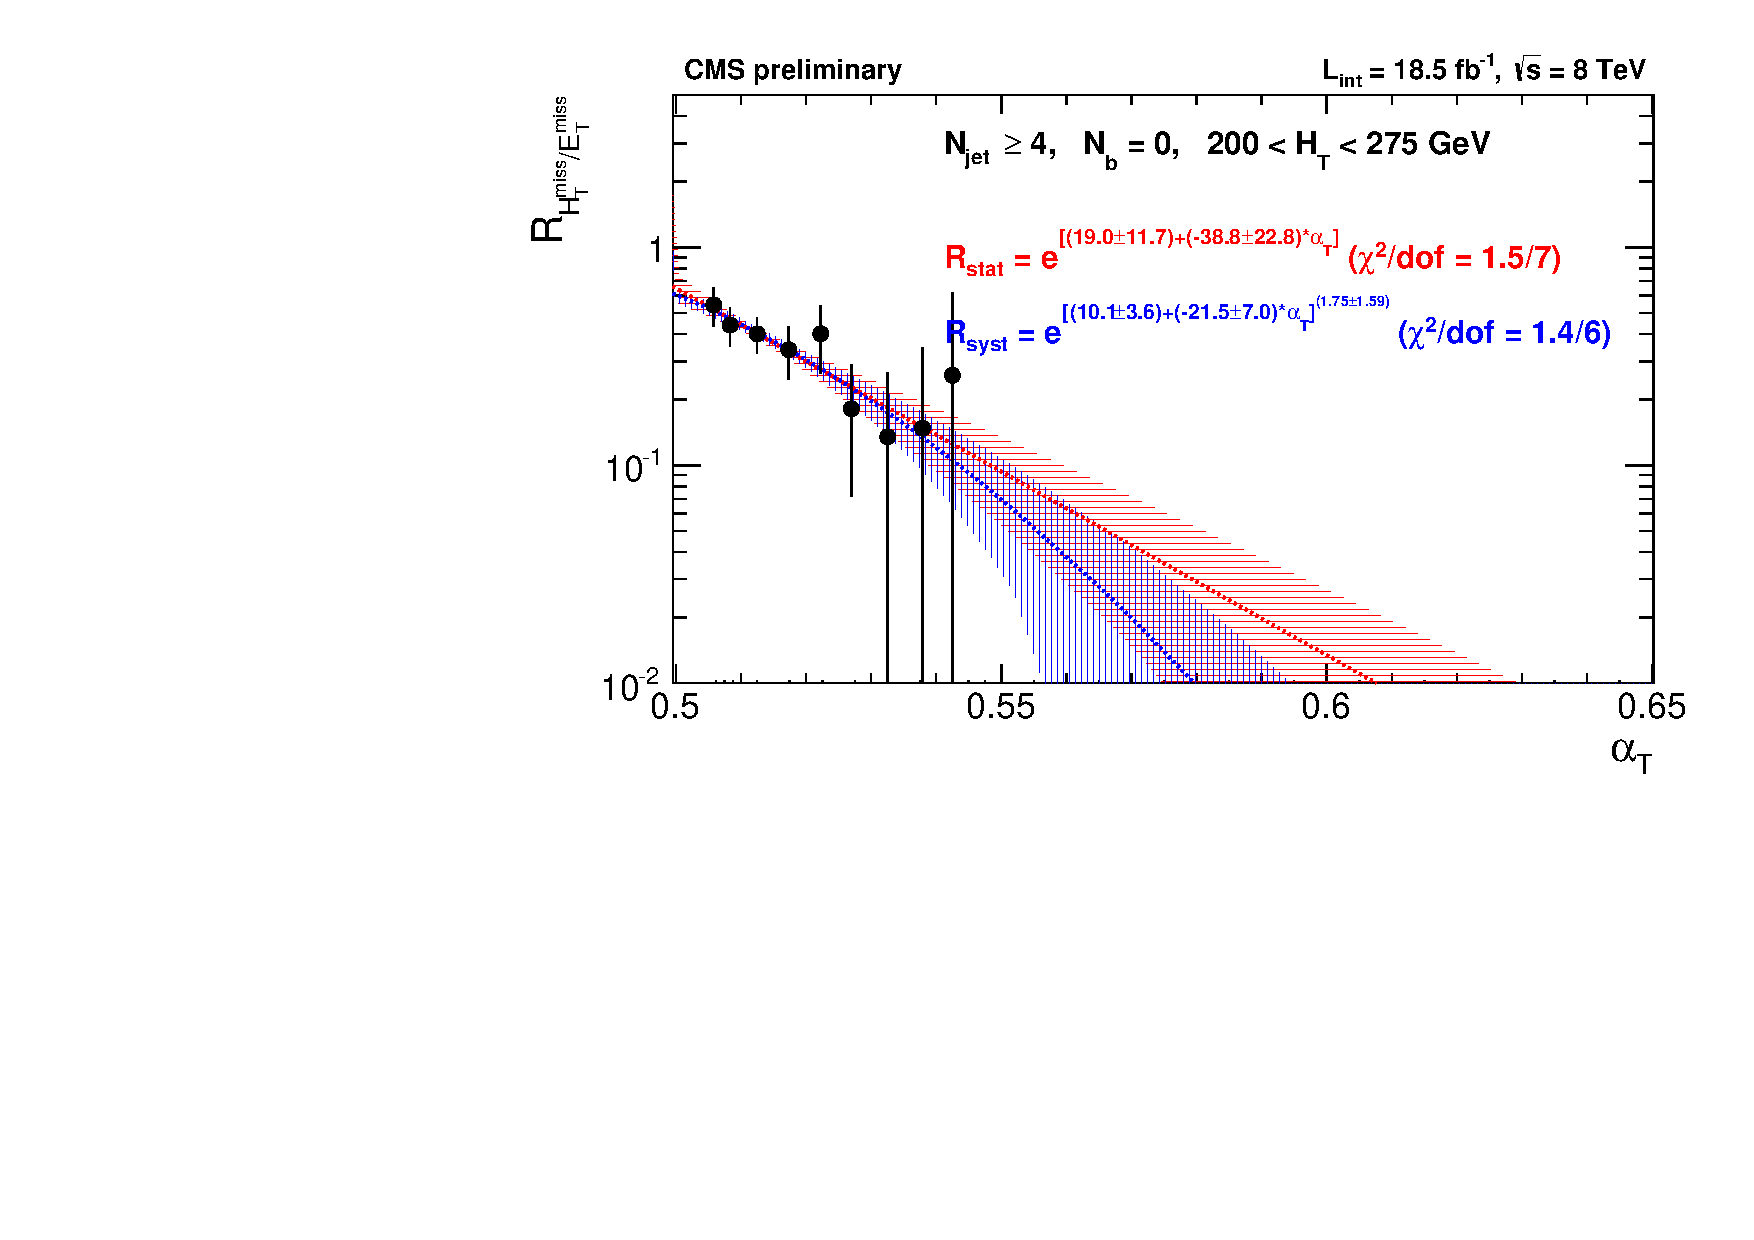
\includegraphics[width=0.5\textwidth]{figures/qcd/ratio_ge4j_eq0b_200}
  } \\
  \caption{Ratio of multijet events passing and failing the \mhtmet
    requirement as a function of \alphat as measured in data for the
    (a) low and (b) high jet multiplicities in
    the low \HT region ($200 < \HT < 275\gev$). }
  \label{fig:qcd-ratio-data}
\end{figure}

Figure~\ref{fig:qcd-ratio-data} shows the ratio \rmhtmet determined
from 8~TeV data as a function of \alphat for (a) low and (b) high jet
multiplicities in the low \HT region ($200 < \HT < 275\gev$).  Also
shown in each figure is the result of an exponential fit (red solid
line) in a low \alphat sideband. The red band represents the
statistical uncertainties associated with the maximum-likelihood
values of the fit parameters. An alternative fit (blue solid line)
with an additional parameter included as a power term allows for
``deviations'' away from the assumed exponential behaviour. The
maximum-likelihood values for the 3-parameter fits and their
uncertainties (blue band) are propagated through to the predictions,
which are assumed to represent an appropriate systematic uncertainty.

Based on studies of 8~TeV data, the expectation is that the
\HT-dependent \alphat thresholds defined in
Table~\ref{tab:sr-selections} and the requirement of $\bdphi > 0.3$
will be sufficient to reduce the multijet contamination in all bins of
the signal region to the sub-percent with respect to the total
non-multijet background. With this level of suppression, it is
expected that the uncertainty associated with the residual multijet
contamination to be sub-dominant with respect to, and fully aborbed
by, the systematic uncertainties on the non-multijet backgrounds,
which are expected to be at the level of $\sim$5\% or larger. 
However, the cuts inspired by the 8 TeV data analysis will be checked
once sufficient 13 TeV data are available.
